\documentclass[a4paper,12pt]{jsarticle}
\usepackage[dvipdfmx]{graphicx}
\usepackage{here}
\usepackage{url}
\usepackage{lmodern}
\usepackage{textcomp}
\usepackage{latexsym}
\usepackage[fleqn]{amsmath}
\usepackage{float}
% 下の3行のコメントを外すと原稿チェックのための行番号がでる
%\usepackage{lineno}
%\linenumbers
%\modulolinenumbers[5] % 5行ごとに行番号を出す

\begin{document}

%%-----------------------------------------------------------------------
%% 表紙
%%-----------------------------------------------------------------------
\begin{titlepage}
\begin{center}
\fontsize{14pt}{0pt}\selectfont
\par
千葉工業大学\\
修士学位論文

\vspace{3cm}

\fontsize{14pt}{3pt}\selectfont
\par
%% タイトル
\Huge 時空間永続証明のための\\
\Huge ブロックチェーン履歴交差法の検討\\

\vspace{7cm}

\fontsize{14pt}{1cm}\selectfont
\par
所属専攻:電気電子情報工学専攻
\vspace{0.25cm}

\fontsize{14pt}{0pt}\selectfont
\begin{tabular}{lll}
%% 氏名および学生番号
学籍番号・氏名:1972042 & 柳原 貴明 \\
\end{tabular}

\vspace{1cm}

\par
指導教員:藤原 明広 准教授

\vspace{1cm}

\par
%% 提出日
提出日 令和3年 3月dd日
\end{center}
\end{titlepage}

\normalsize
\pagenumbering{roman}


%%----------------------------------------------------------------------
%% 概要
%%----------------------------------------------------------------------
\section*{概要}
最後に書く                 


\newpage
%%----------------------------------------------------------------------
%% 目次
%%----------------------------------------------------------------------
\tableofcontents
\newpage

%%----------------------------------------------------------------------
%% 本文
%%----------------------------------------------------------------------
\pagenumbering{arabic}

%%----------------------------------------------------------------------
\section{序論}
%%----------------------------------------------------------------------

(仮)
Bitcoinを代表とする(パブリックな) ブロックチェーンは,世界中に散在するコアノード同士で,
取引データやブロックを転送するため頻繁に共有し合っている.
地理的に近いコアノード同士では通信遅延時間の影響は少ないが,
遠距離のノードにブロックを転送する場合,数十秒〜数分の通信遅延が起きることが知られている.

この遅延により,Proof of Work( PoW )によるブロック生成時間を十分遅くする必要がある
この理由によりビットコインではブロック生成時間が10分になるように制御されている.

この遅延時間により,単位時間に処理可能な取引量が少なくなる.これは「スケーラビリティ問題」として知られている. 
この問題を解決する方法の一つとして,地理的に近いコアノード同士でドメインを自律的に形成し,
ドメイン毎に独自のブロックチェーンを管理する方法が提案されている \cite{fujihara1}\cite{fujihara2}.
しかし,各ドメインに存在するコアノードの数が減少するため,
ブロックチェーンの非中央集権性と改ざん耐性が低下する問題があった.
本章では,本研究の背景として現状の動向と先行研究の問題点を挙げ,本研究目的を述べる.


\subsection{背景}
近年,クラウドコンピューティングおけるデータサーバーの仮想化を代表されるような
ストレージやネットワーク,アプリケーションなどの様々な機能が仮想化技術によって提供されています.
データサーバーを管理する企業・組織に依存することになる。
ブロックチェーンので

分散システムには貨幣や資産のようなデータで扱えない決定的な決定的な欠点があります。
(ブロックチェーンが成し遂げたこと)

ソフトウェアシステムの構造(アーキテクチャ)には大きく「集中システム」と「分散システム」
の2つがあります。
図のように集中システムは1つの中心があり,そこに他のコンピュータが接続する形になっており,

分散システムは,複数のコンピューター同士が接続し合って形成されます.
システムによっては、分散システムと集中システムを組み合わせることもあり,
状況に応じて適切な構造を採るように工夫されています.

集中システムと分散システムそれぞれの長所・短所は表ーーーの通りであり
以下のようになる。
比較すると、この2つは正反対の性質を持つ構造だと分かります.

集中システムでは,中心にあるコンピューターが動かなくなるとシステム全体が
停止(システムダウン)してしまう「単一障害点」と呼ばれるマシンが存在したり、
維持管理にコストが掛かってしまったりする欠点があるもののシステムの柔軟性や
一貫性を維持するのが比較的、容易である長所があります.
またなりよりもシステムにおけるデータの完全性を維持できる

データの完全性は、データにかけているころ所や間違っていることがない性質の

分散システムはシステムにおける処理を多くのコンピューターで
分担するためコストを削減することができ、単一障害点がないことでシステムダウンする可能性がとても低くなります.
加えて,計算能力を高めていくことが可能です.

ネットワークに接続している多くのコンピューターの計算能力を利用できるため全体の計算能力が高くなると同時に、
接続するコンピュータを増やすことで、その計算能力を徐々に大きくすることも可能です.

今では多くの人々が高性能のPCやスマートフォンなどを持つようになっているため、
それらが接続し合って大きな計算能力を実現できるのうになりました.

また低コストかつダウンしないシステムであれば、紙幣資産のような重要なデータを扱うことが
できるように思えます.

(ブロックチェーンが成し遂げたこと)
しかし、分散システムには
貨幣や資産のような重要データを扱えない決定的な欠点があります。
貨幣や資産のデータがネットワーク上のコンピューターによって異なっていると、どのデータを信じれば良いか分からなくなり、
データへの信頼性がなくなってしまいます。

このような状況では、重要なデータを扱うことは出来ません。
そのため、貨幣や資産などのデータはこれまで、完全性を維持しやすい集中システムを中心に扱われてきました。

しかし、すでに紹介した通り、集中システムには単一障害点という”急所”があり情報が一カ所に集まっています。
このことは長所であるものの、維持管理するために必要な技術やコストが高くなることや、情報が集中することによるプライバシーの問題
を浮き彫りにしてしまいます。

そこでプライバシーの問題が小さくコストを抑え計算能力の高い分散しシステムで、集中システム程の利便性を持つことができれば
両者のいいとこ取りができます。
そこでブロックチェーン技術です

ブロックチェーン技術は多くのメリットを持つ
分散システムで集中システムのようにデータの完全性を維持するための技術
として開発されたと見ることができる
その意味では、分散システムの可能性をさらに拡張するために技術であり、
新たな扉を開いた技術として熱い視線を浴びることとなったのです。

\subsubsection{ブロックチェーンの構造}

ブロックチェーンは「ブロック」と呼ばれるデータを数珠状につないだ形を
しており、ブロックを要約したブロックに取り込むことで全体の整合性を取っております。

\subsubsection{ブロックチェーンの非中央集権性}

\subsubsection{ブロックチェーンの改ざん耐性}

 本研究では,独自のブロックチェーンを管理する複数のドメイン間で
定期的にブロックチェーンの状態を共有することで,互いのブロック
チェーンにヒステリシス署名を書き込み合う履歴交差法を提案する.
提案手法について理論的および実験的観点から,その有効性を評価した.
まず,提案法による改ざん耐性の向上比率について理論的に評価した.
次にドメイン間で自律的に通信を行うプロトコルを設計し,実際に
提案法を実行するノードを実装した.
その上で,実際に履歴交差法にかかる遅延時間を計測し,その成功率
も実験的に評価した.
その結果,理論的に改ざん耐性向上比率が高いことと,実験的に
成功率が高いことを確認した.

この遅延時間により,単位時間に処理可能な取引量が少なくなる.これは「スケーラビリティ
問題」として知られている. 
この問題を解決する方法の一つとして,地理的に近いコアノード同士でドメインを自律的に形成し,
ドメイン毎に独自のブロックチェーンを管理する方法が提案されている \cite{fujihara1}\cite{fujihara2}.
しかし,各ドメインに存在するコアノードの数が減少するため,
ブロックチェーンの非中央集権性と改ざん耐性が低下する問題があった.
そこで本研究では,ドメイン間で定期的にブロックチェーンの状態を共有し,
互いのブロックチェーンにヒステリシス署名\cite{suzaki}を書き込み合う履歴交差法を用いることで,
スケーラビリティ問題の解決を検討する.
まず,履歴交差法によって改ざん耐性向上比率がどの程度向上するかを理論的に評価した.
次に,ドメイン間で自律的に通信を行うプロトコルを設計し,実際に提案法を実行する
ノードを実装した.
その上で,実際に履歴交差法にかかる遅延時間を計測し,その成功率
も実験的に評価した.
その結果,理論的に改ざん耐性向上比率が高いことと,実験的に成功率が高いことを確認した.

\subsection{本研究の目的}
研究目的

\newpage
%%----------------------------------------------------------------------
\section{関連技術動向と関連研究}
%%----------------------------------------------------------------------
\subsection{関連技術動向}
\subsubsection{Bitcoin}
Bitcoinはデジタルマネーエコシステムの基礎となるコンセプトと技術の集合体です。
Bitcoinネットワークの参加者間で、価値の保有と転送がBitcoinという名の通貨単位で行われます.
ユーザー間の通信は主にBitcoinプロトコルに基づいて、インターネットを通じて行われます。
Bitcoinのプロトコルスタックはオープンソースとして利用可能であり、
ノートパソコンからスマートフォンまで、様々なデバイス上で動作します。

ユーザーはネットワークを通じてbitcoinをやり取りすることで、従来の通貨で行うほぼ全てのこと、つまり
物品の売買から個人や組織への送金、融資まで行うことが可能になります。bitcoin自体も売買が可能であり
、専門の両替機関で他の通貨とも両替することも可能です。bitcoinは高速かつ安全であり、国境を越えて取
引が可能であることから、ある意味でインターネットに使うための最適な通貨ともいえます。
伝統的な通貨と異なりbitcoinは完全に仮想的なものです。物理的なコインは存在せず、またデジタルコイン
自体が存在するわけでもありません。コインは「送信者から受信者へある一定量の額面を移動させる」という
取引(トランザクション)の中で暗に示されるものです。

Bitcoinのユーザーはトランザクションの所有権を証明する鍵を所有し、そのトランザクションの中に記載さ
れた額面を使用したり新しい所有者に送金することができます。 

この鍵はそれぞれの利用者のPC上の電子財布(ウォレット)に保持されます。 
この鍵の保有がbitcoinを使用する唯一の条件であり、そのコントロールは各ユーザーにゆだねられています。

Bitcoinは分散されたpeer-to-peerのシステムであり、何らかの"中央"サーバや管理者が存在するものではありません。

bitcoinは取引の過程で行われる"マイニング"と呼ばれる数学的な解を見つけ出す競争により新たに生み出されます。

どの(フルプロトコルスタックを動作させている)Bitcoinネットワーク参加者も、
自身のコンピューターリソースを用いて取引の記録処理と検証処理を行うことでマイナーとなることができます。

平均して10分に1回の頻度で誰かが数学的な解を見つけることで取引が検証され、
その解の発見者にはbitcoinが新たに与えられます。

つまるところbitcoinのマイニングとは、中央銀行が行う必要があった通貨の発行と決済の機能を、
世界的な競争で代替したものなのです。
Bitcoinプロトコルにはマイニングの機能を規定するアルゴリズムが組み込まれています。
マイナーが行わなければならないタスクの難易度は、マイナーの数(またはCPUの数)が変動しても
平均的に10分に1回ほど解が見つかるように自動的に調整されます。 

またプロトコルではbitcoinが新たに発行される頻度は4年毎に半減されるように規定されており、
またbitcoinの総発行量は2100万bitcoinを超えないように規定されています。
結果、bitcoinの流通数は容易に予想可能で2140年に2100万に到達するカーブを描くことになります。

長期的にbitcoinの発行レートが減少していくため、bitcoin通貨はデフレーション傾向となります。

さらに、予期された通貨発行レートよりも多く通貨が"発行"されることがないため、
インフレーション状態になることはありません。

Bitcoinはプロトコル名でもありネットワーク名でもあり、
さらには分散コンピューティングのイノベーションの名称でもあります。
通貨としてのbitcoinはこのイノベーションの単なる最初の応用であるだけです。
開発者の視点から、Bitcoinを通貨のインターネット、
つまり分散コンピューティングによって価値やデジタル資産の所有権のセキュアなやりとりを
行うためのネットワーク基盤と考えています。Bitcoinは見た目よりも
大きな可能性にあふれているのです。
この章では主な概念と用語を説明することから始め、必要なソフトウェアを用意し、
単純な取引の中でbitcoinを使ってみます。
その後の章でBitcoinが動作する技術的な部分を明らかにし、
Bitcoinネットワークとプロトコルの仕組みを見ていきます。

\subsubsection{集中システムと分散システム}



\subsubsection{分散台帳技術}


\subsubsection{ブロックチェーン}

ブロックチェーンは2008年に「Satoshi Nakamoto」という仮名の人物
ないし集団が発表がたBitcoinの基幹技術として生まれ、現在は主に仮想通貨としての活用を目指す技術として注目を浴びている.

ブロックチェーンは2008年,匿名の開発者サトシ・ナカモトにより、
デジタル通貨システム「ビットコイン」を実現するための分散タイムスタンプとして提案された.

ビットコインは,管理者のいない環境下で電子的に表現されたコインの制御権の移転,
すなわち送金を実現することを目標に設計されている.
送金の取引は入金(入力)と出金(出力)の間の関係を記述するが,
ビットコインでは,未使用の取引出力がコインであるとするいわゆる

UTXO(Unspent TX Output)構造(図 -1)を用いて電子コインのディジタルデータ形式を定義している.
この構造は,適切な秘密鍵を用いて取引にディジタル署名できる主体だけが送金できることを保証するが,
署名の検証に必要な情報(公開鍵)をデータ構造の中に埋め込み,
公開鍵のメッセージダイジェスト(ハッシュ値)をコインの送金の宛先とすることで,
まったく関係のない第三者でも公開鍵の正当性を確認でき,
取引の形式的な正しさを検証可能にした点で画期的である.

\subsubsection{ビットコインにおけるブロック構造}

\subsubsection{P2Pネットワーク [peer to peer sysytem]}
全てが同じである複数プロセスによって構成される.

P2Pシステムで行われるべき

\subsubsection{Proof of Work (PoW)}
difficultyターゲットを満たすSHA256のアルゴリズムに対し、解を見つけなければなりません。

\subsubsection{暗号学的ハッシュ関数} %(参考@分散システム31第2班)
暗号の利用方法の1つに,メッセージの完全性を確認するための情報であるメッセージダイジェストと呼ばれる固定長のビット列を生成するものがある.
任意の長さのメッセージから固定長のビット列を生成する暗号アルゴリズムは,暗号学的ハッシュ関数と呼ばれる.

暗号学的ハッシュ関数は,以下の性質を持つことが特徴である.

\item 原像計算困難性
\item 第2原像計算困難性
\item 衝突困難性

原像計算困難性とは,ハッシュ値$h$が与えられたとき,$ h = hash(m)$となるような任意のメッセージ$m$を探すことが困難な性質である.

第2原像計算困難性とは,入力$m1$が与えられたとき,$ hash(m1) = hash(m2)$ となるようなもう1つの入力$m2$($m1$とは異なる入力)を
見つけることが困難である性質である.

衝突困難性とは,$hash(m1)= hash(m2)$となるような2つの異なるメッセージ$m1$と$m2$の組を探すことが困難である性質である.
これらの性質によって,2つのメッセージに対するダイジェストが同じである場合,メッセージが同一である可能性が高いことを意味する.

また,逆にダイジェストが異なる場合は,メッセージは異なるものであることを意味する.


送信者から送られた文書が,正しく送信者が作成したものであるかは,文書全体が送信者の秘密鍵で暗号化されていれば確実である.
しかし文書全体を公開鍵暗号方式で暗号することは効率面から難しいし,またその必要のない場合が多い.
そこで,文書全体を暗号化するのではなく,文書の完全性を保証する情報を秘密鍵で暗号化して添付することが多い.

それを電子署名(デジタル署名)という.

文書の完全性を保証する情報としては,メッセージダイジェストが用いられる.
メッセージダイジェストは入力文書の大きさのよらない固定長の情報(ハッシュ値)であり,以下の特徴を持つ.

\item メッセージからメッセージダイジェストが簡単に計算できる.
\item メッセージダイジェストからメッセージを見つけることは出来ない.
\item メッセージから同じメッセージダイジェストが生成される別のメッセージを見つけることはできない.
\item メッセージを1ビットでも変更すれば,メッセージダイジェストは全く異なる値になる.

このような特徴を持つ

\subsubsection{公開鍵暗号方式}

\subsubsection{履歴交差法}
ヒステリシス署名の証明力はこうした
ヒステリシス署名つき文書が作成したエンティティの電子文書が署名を作成したエンティティの手を離れ,
他のエンティティの電子文書におけるヒステリシスとして署名に織り込まれた時に,さらに飛躍的に向上すると考えられる.
図3

それは,第一には,こうした履歴情報の交差によりヒステリシス署名が拡散することじゃ,「過去の電子署名」を偽造しようとする
ときの作業量を鼠算的に拡大させる空であり,第

\subsubsection{電子署名}
通常の電子署名は秘密鍵が漏洩することによる改ざん
が可能であり,改ざんされたことの検知も不可能である.

一方,ヒステリシス署名では,電子
署名が入れ子構造になって署名がされている為,署名の改ざんを行う為には,改ざんした内容
以降の全ての入れ子構造になった署名を改ざんする必要があり,改ざんが著しく困難になる.
また,部分的に改ざんされた場合は,入れ子構造を検証することで,改ざんの検知も可能になる.
これはPoWに代わる改ざん耐性技術としてブロックチェーンが注目を集める前から知られており,
過去のデータ等を改ざん耐性を持たせて保存することができる.

\subsubsection{ヒステリシス署名}

ヒステリシス署名過去の署名履歴を取り込みながら署名生成を行う方式である.

ヒステリシス署名\cite{suzaki}とは,通常の電子署名に連鎖する入れ子構造を持たせることで,
その改ざん耐性を向上させる技術である.
図\ref{fig:hysteresis}にヒステリシス署名の構造を示す.
1つ前のヒステリシス署名$S_{n-1}$を暗号学的ハッシュ関数にかけたハッシュ値$H(S_{n-1})$
と一緒に保存したい$m$個のデータ($B_{D_1}, \cdots, B_{D_m}$)のハッシュ値
($H(B_{D_1}), \cdots, H(B_{D_m})$)を追加する.この全体の署名$S_n$を更に追加して生成された
ものがヒステリシス署名となる.

これにより有効期限のが切れた電子証明書に対応する電子署名であっても,有効期限内の電子署名書により
真正性が保証された電子署名空から連鎖構造を辿ることで,結果として真正性を証明可能となる.

なお通常の署名方式では,署名方式では,署名対象となるメッセージと電子署名とを組みにして相手の(検証者)に送るが,
ヒステリシス署名では,それに加えてひとつ前の署名結果のハッシュ値も合わせて送ることが可能になる.

時間情報を文書に織り込むのではなく,署名者が過去に関わった署名付き電子文書の圧縮データを次々に織り込んで行くことである.


%ヒステリシス署名は、直前に生成された電子署名のハッシュ値を取り込み,電子署名間に連鎖構造を持たせる
%署名である.これにより有効期限のが切れた電子証明書に対応する電子署名であっても,有効期限内の電子署名書により
%真正性が保証された電子署名空から連鎖構造を辿ることで,結果として真正性を証明可能となる.

%ヒステリシス署名とは,過去の署名履歴を取り込みながら署名生成を行う方式である.
%これにより署名間に連鎖構造を築き,暗号ブレイク時にも偽造を困難にする.
%ヒステリシス署名では,n回目の電子署名生成時にn-1回目の署名結果のデータのハッシュ値を作用させる.
%従ってある時でのデータは,当該署名しシステムを使用開始してからのすべての署名履歴が影響した値となっている

%なお通常の署名方式では,署名方式では,署名対象となるメッセージと電子署名とを組みにして相手の(検証者)に送るが,
%ヒステリシス署名では,それに加えてひとつ前の署名結果のハッシュ値も合わせて送ることが可能になる.


%電子署名技術が署名鍵の作成と解読における
%計算量の非対称性に依存する限り,コンピュータ技術の進歩により,
%暗号のブレイク状況,すなわち署名生成鍵を持っているエンティティが
%本来の鍵所持者以外にも存在するという可能性を確率的に有意とみなさざることを得なくなる
%状況が生じるこことは避けられない.
%これが電子署名アリバイ問題における基本的な状況設定である
%こうした状況でアリバイを実現するときの基本的な方法は,署名対象文書にその時間情報を織り込んで
%署名することである.

%しかし,そうした時間情報を再現可能なデータを織り込む限りでは,過去のに利用可能であった
%時間情報データを使って「過去の電子署名」偽造することは一般に可能となってしまう

%そしてこうした「過去の電子署名」偽造の可能性が存在する限り,調停者は電子署名のアリバイを承認することも崩すことも出来ない.


\subsubsection{ブロックチェーンにおけるスケラビリティ問題}
ブロックチェーンにおけるスケーラビリティ問題は,



\subsection{関連研究}
\subsubsection{BBc-1}

BBc-1\cite{saito}は,プライベートな取引データを履歴交差により改ざん耐性を持たせて
保存する (ブロックチェーンではない) 分散台帳技術である.ノードの実装も行われており,
その有効性が実験的にも確認されている.
BBc-1では,取引データにヒステリシス署名を追加する.
ヒステリシス署名を取引データに付けて,ドメイン間でデータを共有することで改ざん耐性を
高めている.また,PoWによる改ざん耐性の向上を行わない為,エネルギーコストは低く済む
特徴がある.しかし,改ざん耐性がどの程度向上したかを理論的に評価しにくいことも知られ
ている. 

\subsubsection{bloXroute}
bloXroute \cite{bloX} では,P2Pネットワーク上で取引データやブロックの共有速度を早める
為に,構造化されたネットワークを(Layer0と呼んでいる)上位ネットワークに構築する提案を
行っている.

ドメイン間で相手を信用することなく通貨を交換できる技術として,Atomic Swap \cite{atomicswap}
が知られている.
マルチホップ通信の問題を解決するための手法である移動シンク方式について述べる.

\newpage
%%----------------------------------------------------------------------
\section{ブロックチェーン履歴交差法}
%%----------------------------------------------------------------------
\subsection{提案手法}
\label{teian}

本研究において提案するP2Pネットワークの構成を図 \ref{fig:p2p}に示す. 
%
%
P2Pネットワークは,Layer0と1の2種類から構成される.
Layer1は通常のブロックチェーンを共有するP2Pネットワークである.固有の
ブロックチェーンを共有しているP2Pネットワークに所属するノードの集合の
ことをドメインと呼ぶ.今回の提案では,複数のドメインが互いに履歴交差法
によりブロックチェーンの「指紋」をヒステリシス署名として共有することで,
全ドメインの改ざん耐性の向上を目指す.Layer1では,各ドメイン 
($D_1, D_2, \cdots, D_m$) が独自のブロックチェーンを管理する.
Layer0は,Layer1を代表する中心コアノード同士がLayer1とは異なる,Layer0
のP2Pネットワークにより相互接続している.
ここでは簡単の為,各ドメインの中心コアノードは1つとしているが,一般に
複数あっても構わない.
このように上位層としてLayer0を付与することは,別の手法でも同様に提案さ
れている\cite{bloX}.

\subsubsection{ブロック構造}
提案するブロックの構造を図\ref{fig:block}に示す.
%
\begin{figure}[h]
  \begin{center}
    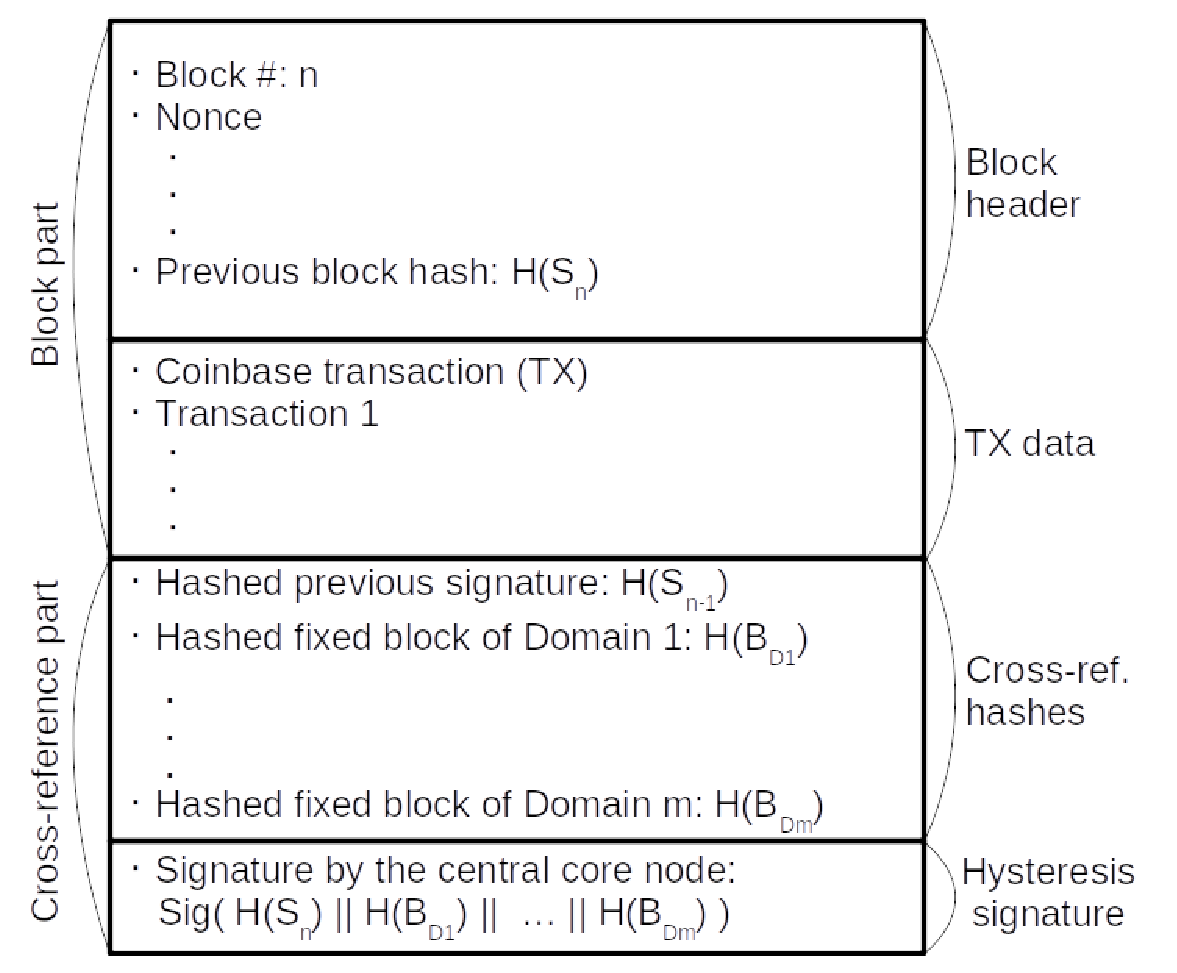
\includegraphics[width=70mm]{pht/block_structure.eps}
  \end{center}
  \caption{提案するブロック構造}
  \label{fig:block}
\end{figure}
%
従来のブロック構造の後ろに履歴交差部 (Cross-reference part) を追加
している.また履歴交差部に書き込むヒステリシス署名は,Layer0を介して
共有する.

\subsubsection{履歴交差法}
履歴交差法の動作を図\ref{fig:cross-ref}に示す.
%
\begin{figure}[h]
  \begin{center}
    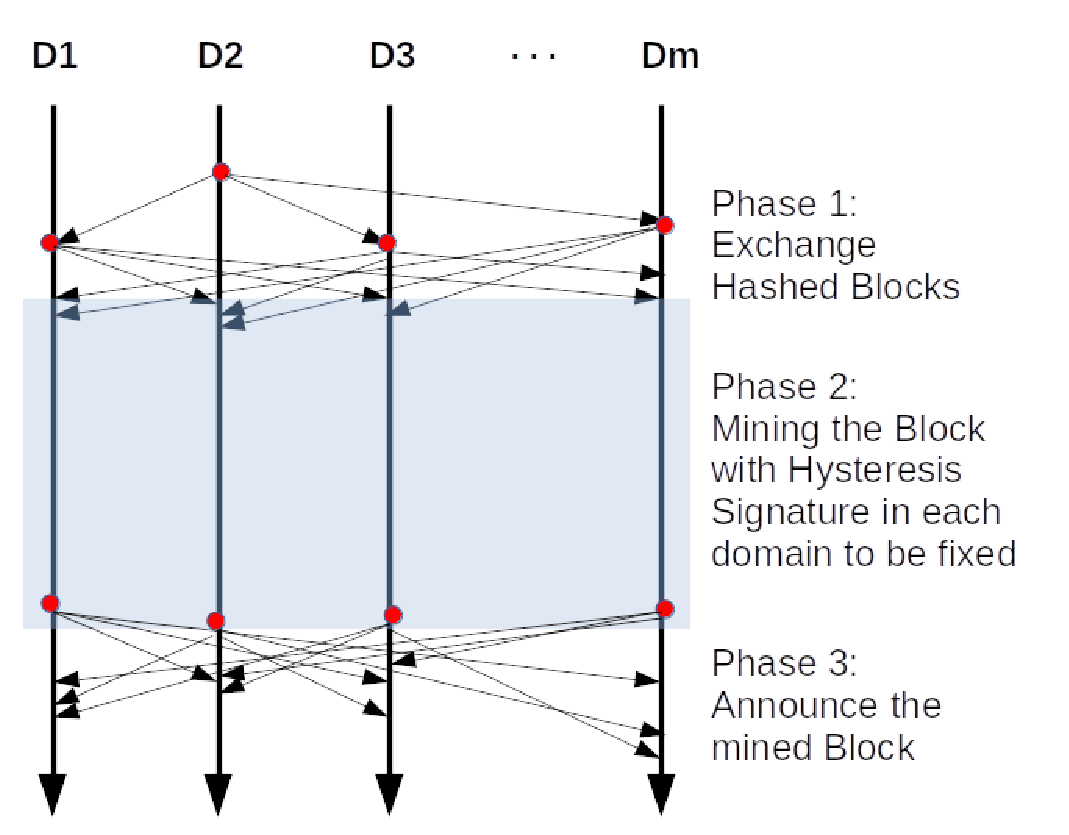
\includegraphics[width=70mm]{pht/time_sequence-algorithm1.eps}
  \end{center}
  \caption{提案する履歴交差法}
  \label{fig:cross-ref}
\end{figure}
%
全体の動作は,次の3つのPhaseから構成される.以下にその流れを簡単に
説明する.

\hspace{5mm}
%
\begin{enumerate}
\item Phase1では,ドメイン間で$l$-確定ブロック (最新のブロックから 
      $l$ 個前のブロック) を含むメッセージをドメインを代表する
      中心コアノード同士で互いに送り合う(ただし$l$は正の整数).

\item Phase2では,各ドメインが届いたメッセージを用いて図\ref{fig:hysteresis}
      のヒステリシス署名を行い,各ドメインが独立に署名を履歴交差部に書き込む
      為のマイニングを行う.

\item Phase3では,マイニングし終えたブロックが,$l$-確定ブロックになったこと
      を他のドメインにブロードキャストして報告する.
\end{enumerate}
%
\hspace{5mm}

履歴交差法を実現する分散アルゴリズム\cite{manabe}を設計した.
その詳細を図 \ref{fig:algorithm1},\ref{fig:algorithm2}に示す.
%
\begin{figure}[h]
  \begin{center}
    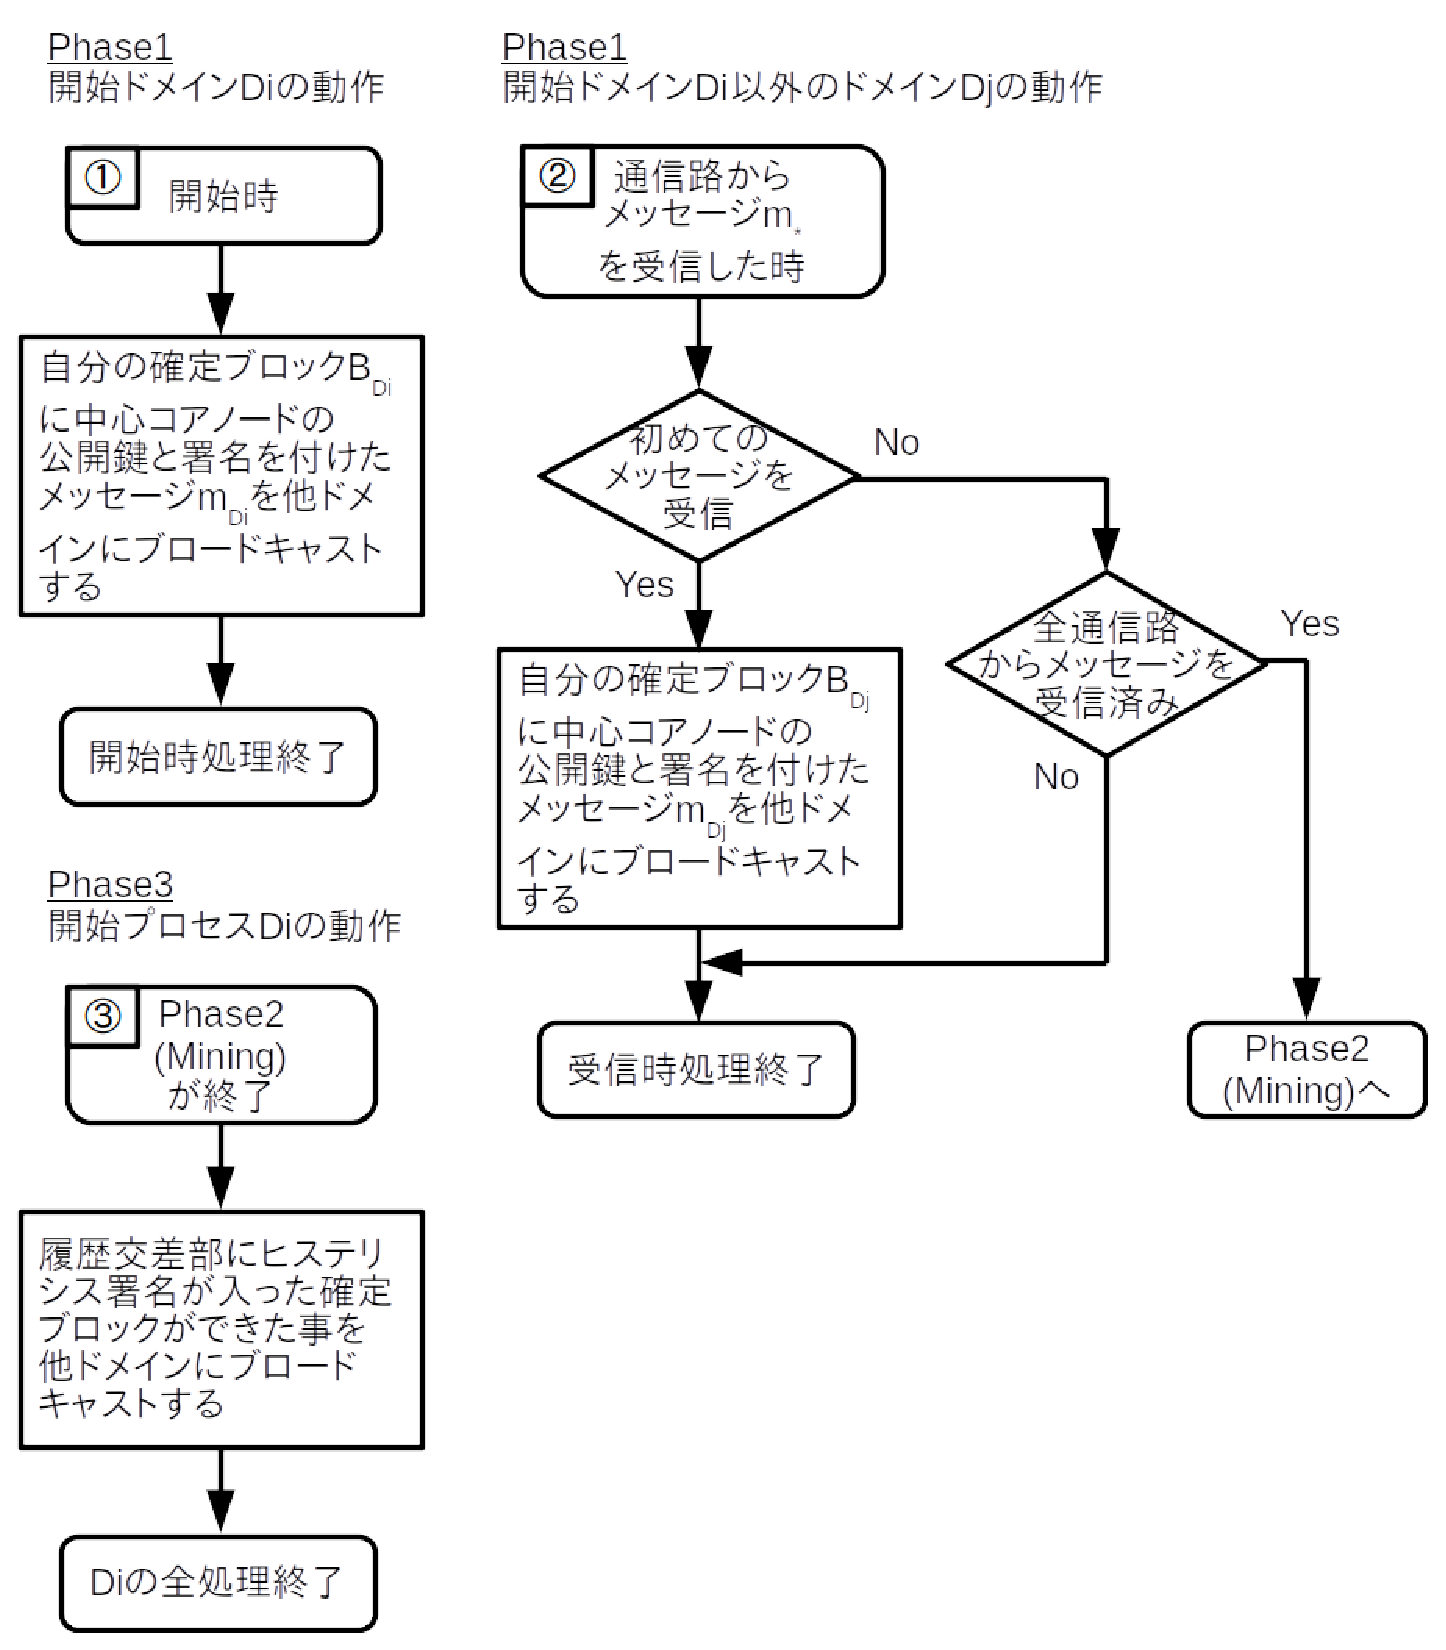
\includegraphics[width=85mm]{pht/flow_chart-algorithm1.eps}
  \end{center}
  \caption{アルゴリズム1(Phase 2はLayer1における通常のマイニング作業を行うだけ
	である為,省略した.)}
  \label{fig:algorithm1}
\end{figure}
%
%
\begin{figure}[h]
  \begin{center}
    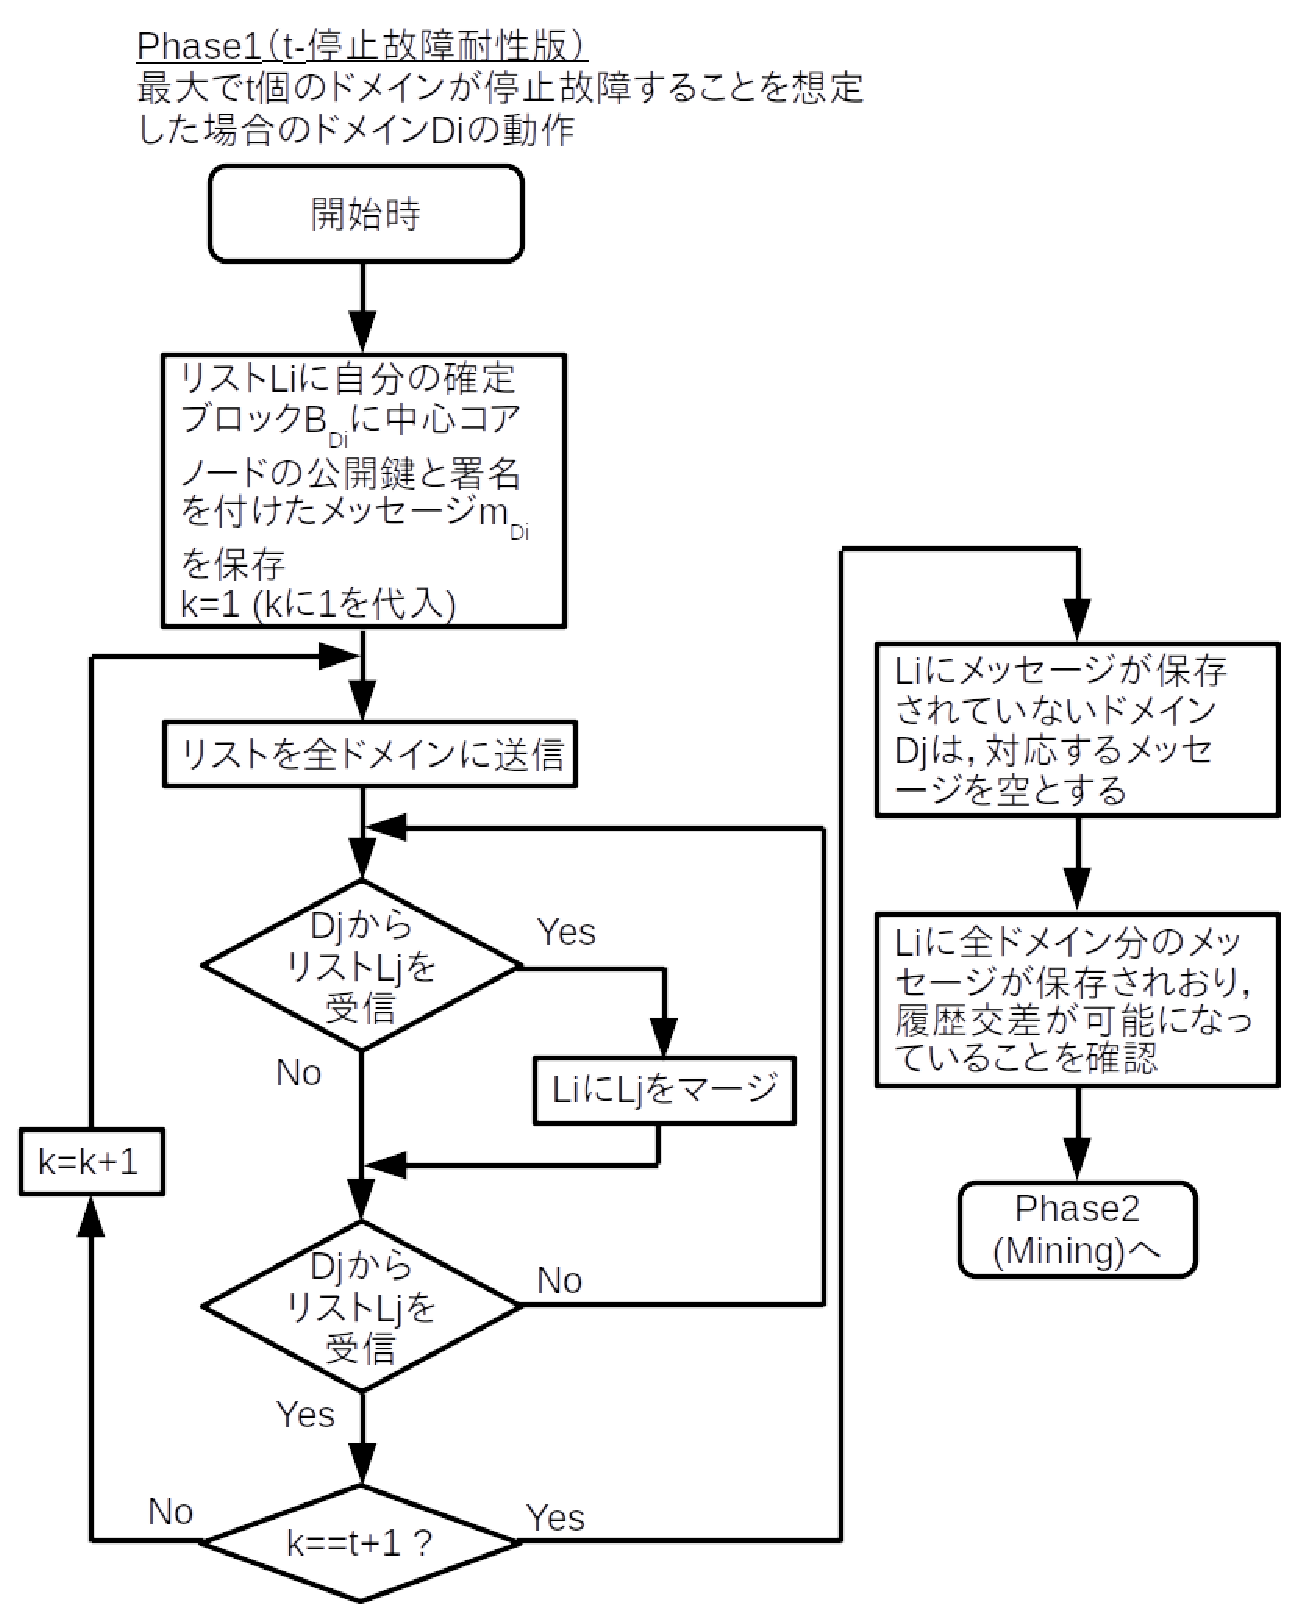
\includegraphics[width=85mm]{pht/flow_chart-algorithm2.eps}
  \end{center}
  \caption{アルゴリズム2(Phase 1のみを記述.その他のPhaseはアルゴリズム1と共通.)}
  \label{fig:algorithm2}
\end{figure}
%
 2つのアルゴリズムが正しく動作する前提条件として,次の1〜3が挙げられる

\hspace{5mm}
%
\begin{enumerate}
\item 中心コアノード同士が作るP2PNWは同期システムである.また,その構造は完全グラフとする.

\item 中心コアノードは正しくアルゴリズムを実行し, 互いに必ずブロックを転送する.

\item アルゴリズム1では,全ての中心コアノードに故障停止がない場合に動作する.
	
\item アルゴリズム2では,$t$-故障停止がある場合を想定する.
      つまり,最悪$t$個の中心コアノードが故障停止に陥った場合でも動作する.
\end{enumerate}
%
\hspace{5mm}
分散アルゴリズムの効率は,通信計算量と時間計算量で評価することが一般的である.
アルゴリズム1が開始してから終了するまでに送信される通信計算量は$O(m^2 \cdot b)$,
アルゴリズム2の通信計算量は$O((t+1)(m^2 \cdot b))$となる.
また動作を行った場合の時間計算量は, アルゴリズム1は, $ T_1 + T_2 + T_3 $,
アルゴリズム2は$ ( t + 1 ) T_1 + T_2 + T_3 $ となる. 
ここで $T_i (i=1, 2, 3)$は,アルゴリズム1においてPhase $i$にかかる時間である.

\newpage

\subsubsection{}


%
\begin{figure*}[h]
    \begin{center}
      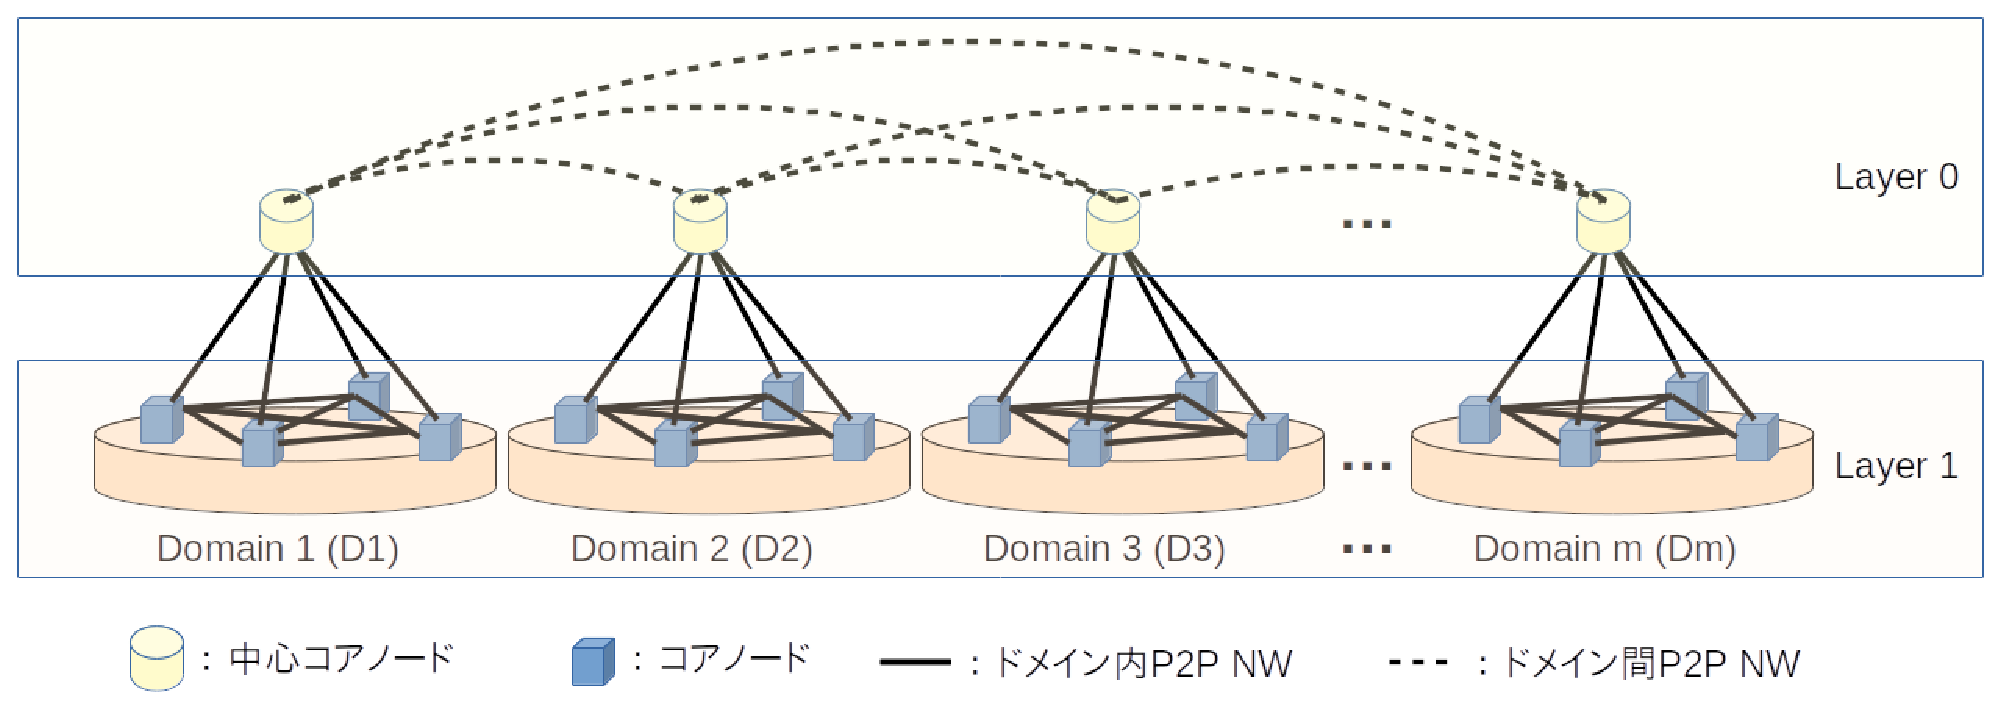
\includegraphics[width=106mm]{pht/p2p_network_image_r1.eps}
    \end{center}
    \caption{P2Pネットワーク}
    \label{fig:p2p}
  \end{figure*}
  %
  %
  \begin{figure}[tb]
    \begin{center}
      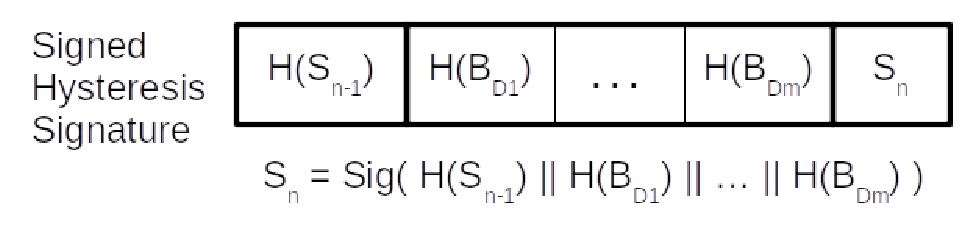
\includegraphics[width=85mm]{pht/hysteresis_signature.eps}
    \end{center}
    \caption{ヒステリシス署名の例}
    \label{fig:hysteresis}
  \end{figure}
  %


\newpage
\subsubsection{}



\newpage
\subsection{評価}
\section{履歴交差法の理論的性能評価}

履歴交差法を行うことで,ブロックチェーンの改ざん耐性が向上することが期待される.ここでは,
改ざん耐性向上比率を定義し,理論的にその比率を評価する.
全ノード数$N$で,ノード$i$のハッシュレートを$h_i$とする.
ここで,ハッシュレートとは, 単位時間あたりに暗号学的ハッシュ関数の計算を行うことができる
回数である.
この時の改ざん耐性は,マイニングに勝利してブロックを生成するのは,ハッシュレートが最も
大きなノードである為,ハッシュレートの最大値で与えられる.
%
\begin{equation}
  \max(h_1, h_2, \cdots, h_N)
\end{equation}
%
ドメイン数が$m$個で,各ドメインに所属するノードの数が$D_m$個の場合を考える.
各ドメインの改ざん耐性は,ドメインに属するノードのハッシュパワーの最大値で
与えられる.
%
\begin{eqnarray}
	A_1 &=& \max (h_{11}, \cdots ,h_{1D1}), \\
	A_2 &=& \max(h_{21}, \cdots ,h_{2D2}), \\
	    & & \vdots \nonumber \\
	A_m &=& \max(h_{m1}, \cdots ,h_{mDm})
\end{eqnarray}
%
このドメインの中でハッシュレートが最大のドメインが履歴交差法に参加する
インセンティブとなるように,全ドメインの中でハッシュパワーが最大のもの
と比較する.
%
\begin{equation}
A = \max(A_1, A_2, \cdots, A_m)
\end{equation}
%
上記の$m$個のドメインで履歴交差法を実行すると,全てのドメインのブロック
チェーンを改ざんしない限り,履歴交差部にヒステリシス署名の証拠が残って
しまう為,改ざんが検出されてしまう.従って,改ざん耐性は全ドメインの
最大ハッシュレートの和で表される.
%
\begin{equation}
	B = \sum_{i=1}^{m} A_i
\end{equation}
%
以上より,ドメイン$i$が履歴交差法に参加することで,期待される改ざん耐性
向上比率$R_i$は次式で表される.
%
\begin{equation}
	R_i = \frac{B}{A_i} > 1 \hspace{5mm} (i=1, \cdots, m)
\end{equation}
%
また,ハッシュレートが最大のドメインが履歴交差法に参加することで期待
される改ざん耐性向上比率$R$は次式で表される.
%
\begin{equation}
	(R_i \ge) R = \frac{B}{A} > 1  \hspace{5mm} (i=1, \cdots, m)
\end{equation}
%
このように,理論的には全てのドメインで改ざん耐性向上率を見積もることが
できる.

ここで,改ざん耐性向上率$R$を見積もる為に,ハッシュレートをランダムに
割り振って乱数シミュレーションを行うことにより,数値的に評価する.
全ノード数を1万とし, ドメイン毎に分割されたノード数を一律 10, 100, 1000
ノードとした場合を評価した.全ノード数を1000万ノードとし,ドメイン毎に
分割されたノード数を一律 10, 100, 1000ノードとした場合の
ハッシュレート $ h_{ij} $ ($i$:ドメイン番号,$j$:ドメイン内のノード番号)を
次式であわらされるパレート分布とした.
%
\begin{equation}
	P(h_{ij}) = \frac{\alpha}{h_{ij}^{1+\alpha}} (h_{ij} > 1).
\end{equation}
%
ここで,$\alpha$はパレート分布のスケールパラメータである.この値が小さい
ほどハッシュレートに格差が大きくなる.一般にハッシュレートはCPUの数に比例
する.CPUをいくつ購入できるかは,ノードを所持する人物ないしはグループの資本
と関係している為,富の分布と相関があると予想できる.この理由により,
ハッシュレートの分布をパレート分布とすることは妥当であると考える.
シミュレーションの実行結果を図 \ref{fig:alpha2}, \ref{fig:alpha3}に示す. 
%
\begin{figure}[tb]
  \begin{center}
    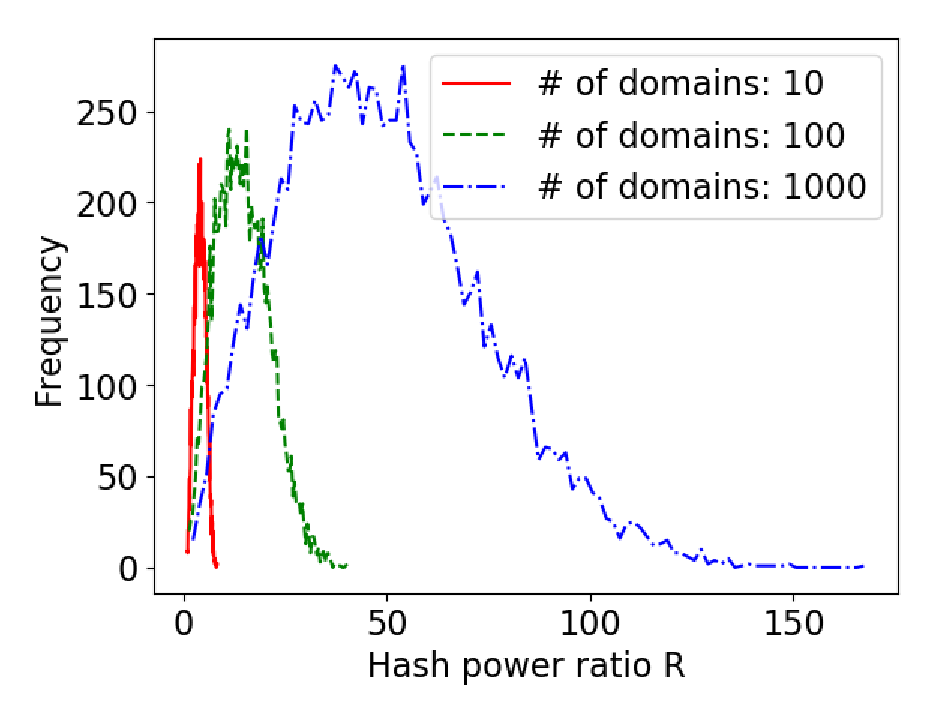
\includegraphics[width=75mm]{pht/hist-comp-R-alpha2.0-m1.0.eps}
  \end{center}
  \caption{改ざん耐性向上比率$R$の確率分布 ( $\alpha=2$の場合 ) }
  \label{fig:alpha2}
\end{figure}
%
%
\begin{figure}[tb]
  \begin{center}
    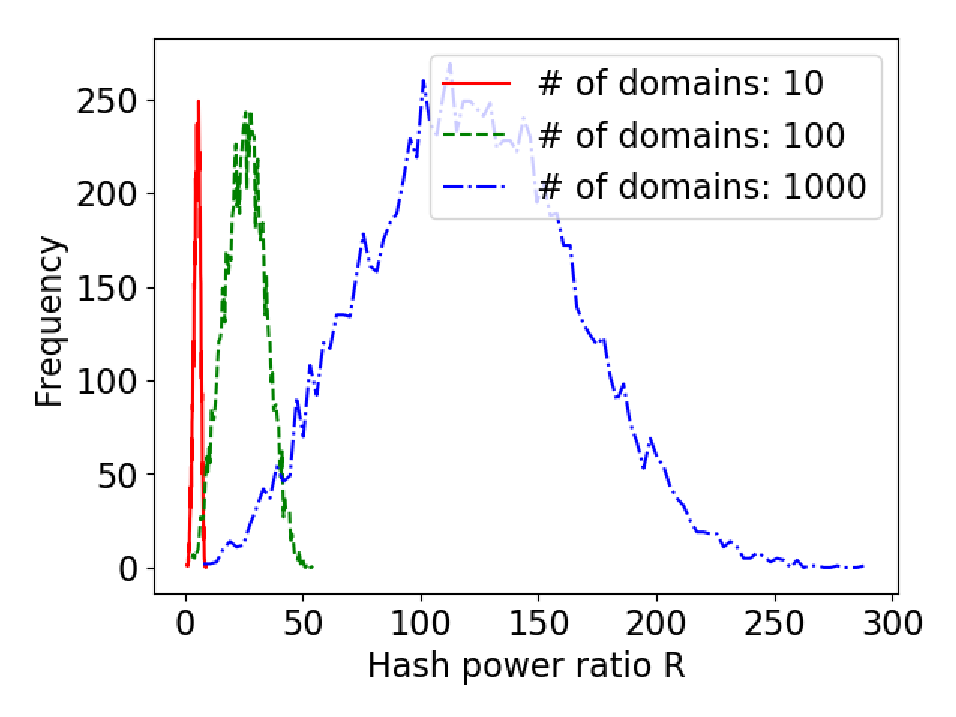
\includegraphics[width=75mm]{pht/hist-comp-R-alpha3.0-m1.0.eps}
  \end{center}
  \caption{改ざん耐性向上比率$R$の確率分布 ( $\alpha=3$の場合 ) }
  \label{fig:alpha3}
\end{figure}
%
一般にドメイン数が増加するほど,改ざん耐性向上比率$R$の分布のピークが
大きい方にシフトすることが分かる.また,ドメイン数が増えると分布の分散
も大きくなることが確認できる.
また図\ref{fig:alpha2}と図\ref{fig:alpha3}の比較により,スケールパラメータ
$\alpha$が小さくなるほど,改ざん耐性向上比率$R$の分布のピークが小さい
方にシフトすることも分かる.

\subsubsection{実験手法}

\section{実験手法}
\label{syuhou}

%
\begin{figure*}[tb]
  \begin{center}
    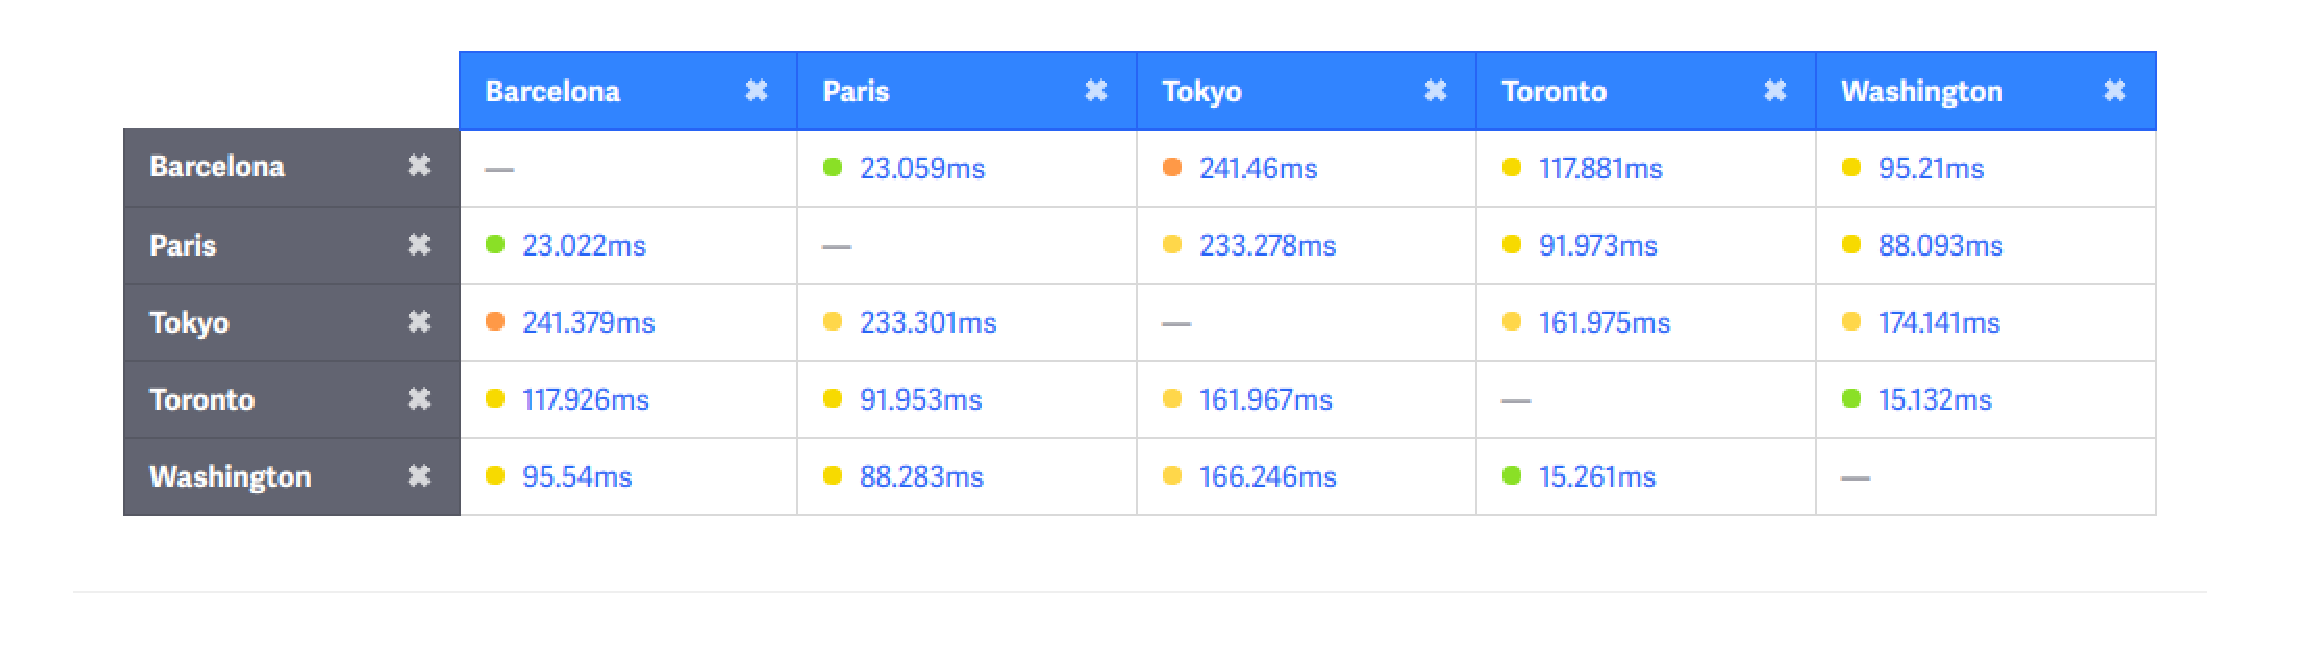
\includegraphics[width=160mm]{pht/Screenshot.eps}
  \end{center}
	\caption{参照したping値\cite{pings}}
  \label{fig:pings}
\end{figure*}
%
\ref{teian} 節の提案手法の実験を行う為に,実際に履歴交差法を行うことが
できるノードを実装した.実装するにあたり,文献\cite{hamatsu2018}を参考
にした.今回は紙面の都合上,アルゴリズム1の実装と実験結果のみを紹介する.

以下にSocket通信によって実装した通信プロトコルを示す.

\hspace{5mm}
%
\begin{enumerate}
\item \textbf{MSG\_REQUEST\_CROSS\_REFERENCE}\\
\hspace{12mm} (履歴交差の依頼 )
\item \textbf{MSG\_ACCEPT\_CROSS\_REFFERENCE}\\
\hspace{12mm}  (履歴交差依頼の承認 )
  \item \textbf{MSG\_START\_CROSS\_REFFERENCE}\\
\hspace{12mm}  (履歴交差の開始号令 )
  \item \textbf{MSG\_CROSS\_REFFERENCE}\\
\hspace{12mm}  (履歴交差を行いたいblock内容の共有 )
  \item \textbf{MSG\_COMPLETE\_CROSS\_REFERENCE}\\
\hspace{12mm}  (履歴交差の完了通知 )
\end{enumerate}
%
\hspace{5mm}

このプロトコルを用いて,履歴交差を1000回行い,各Phaseが修了するまでにかかる
遅延時間分布と履歴交差法の成功率について調査した.
ここで,Layer 0である中心コアノードをドメイン$D_1, D_2, D_3, D_4, D_5$から
それぞれ1つの5ノードからなる状況を想定し,それらの間にP2Pネットワークを
ローカルに構築した環境において実験を行った.
今回は簡単の為に,特定(ドメイン$D_2$)の中心コアノードが2分間隔で履歴交差の依頼を
他ドメインの中心コアノードに行い,履歴交差を開始させることとした.

Phase1では,
ドメイン$D_2$の中心コアノードが履歴交差の依頼 (\textbf{MSG\_REQUEST\_CROSS\_REFERENCE})
を他ドメインの中心コアノードに送信し,ドメイン$D_2$以外の中心コアノードが受信する.
依頼を受信した各ドメインは履歴交差の依頼を了承する返信 (\textbf{MSG\_ACCEPT\_CROSS\_REFFERENCE})
をドメイン$D_2$に送信する.
ドメイン$D_2$の中心コアノードは,他の全てのドメインから了承の返信を受け取ったら,
履歴交差を開始する号令 (\textbf{MSG\_START\_CROSS\_REFFERENCE}) を他ドメインの中心コアノード
に送信し,履歴交差を行いたい$l$-確定ブロックのデータを各ドメインの中心コアノードに
ブロードキャストする (\textbf{MSG\_CROSS\_REFFERENCE}).
同様に号令を受け取った$D_2$以外の中心コアノードは,各ドメインの中心コアノードにブロードキャスト
を行う.個々のドメインの中心コアノードは全てのドメインからの確定ブロックのデータを受取り,
データを暗号学的ハッシュ関数にかけてhash値にする.以上でPhase1は完了となる.

Phase2では,
Phase1の履歴交差部を書き込む為のマイングを行う.今回の実験では,PoWの難易度を5とした.
今回実験を行ったマシンでは,この難易度でブロックを生成するのに10秒程度の時間がかかっている.
履歴交差を行ったブロックが$l$-確定ブロックとなった時点でPhase2は完了となる.

最後にPhase3では,
マイニングを完了したブロックが,履歴交差を行ったブロックから$l$-確定ブロックとなった段階で,
他ドメインの中心コアノードに履歴交差に成功したことをブロードキャストする
 (\textbf{MSG\_COMPLETE\_CROSS\_REFERENCE}).
今回の実験では,$l=3$とした.ブロードキャストを送信した時点でPhase 3は完了となる.

なお,今回の実装には通信遅延を考慮し実装した.
各ドメインがBalcelona,Tokyo,Paris,Toronto,Washingtonにあるとし,履歴交差の依頼を行うドメイン$D_2$はTokyoのものとした.
2020年2月9日のpingのRTTにかかる時間\cite{pings}を参考にすることで,ポート番号でノードを区別して,
sleep関数を利用することで遅延を発生させた.

参考にした文献\cite{pings}は,unixコマンドラインツールのpingを用いており,ウインドウサイズを今回は$64$[Byte]とすると,
pingのRTTをP[ms]から,送信データサイズをB[Byte]に応じた通信遅延Lは,以下の式で表される.
\begin{equation}
  \label{byt}
    L = \frac{BP}{64} [sec]
\end{equation}
送るデータサイズと送り先のポート番号に応じて
通信遅延を発生させた.通信する際におおよそ0.1〜2秒程度の通信遅延Lが発生している.
実際に参照した遅延時間を図\ref{fig:pings},算出したTokyoから150〜500[Byte]のデータサイズを
他のドメインへの送信した際の通信遅延Lの上限値を表\ref{Byte} に示す.

\begin{table}[tb]
  \centering
  \caption{Tokyoからの各ドメインへの通信遅延(小数第2以下は省略)}
  \label{Byte}
  \begin{tabular}{c|c|c|c|c|}
  \cline{2-5}
  [sec]                       & Barcelona &    Paris   &   Toronto  & Washington \\ \hline
  \multicolumn{1}{|c|}{Tokyo} &  0.5〜1.9 &  0.5〜1.9  &  0.3〜1.2  &  0.4〜1.3  \\ \hline
  \end{tabular}
\end{table}

\subsection{実験結果}

前節で解説した通信プロトコルを用いて実験を行った結果として,各Phaseでの
遅延時間の分布を図\ref{fig:phase1}, \ref{fig:phase2}, \ref{fig:phase3}に示す.
%
\begin{figure}[tb]
  \begin{center}
    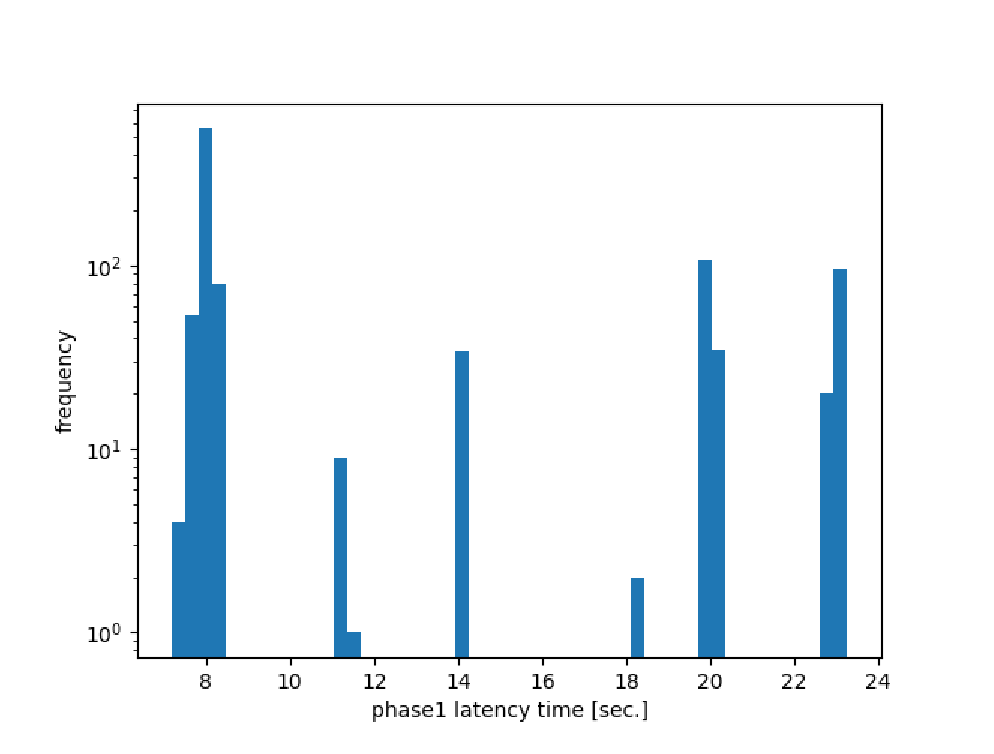
\includegraphics[width=78mm]{pht/phase1-sec-hist.eps}
  \end{center}
  \caption{Phase1の計測時間}
  \label{fig:phase1}
\end{figure}
%
%
\begin{figure}[tb]
  \begin{center}
    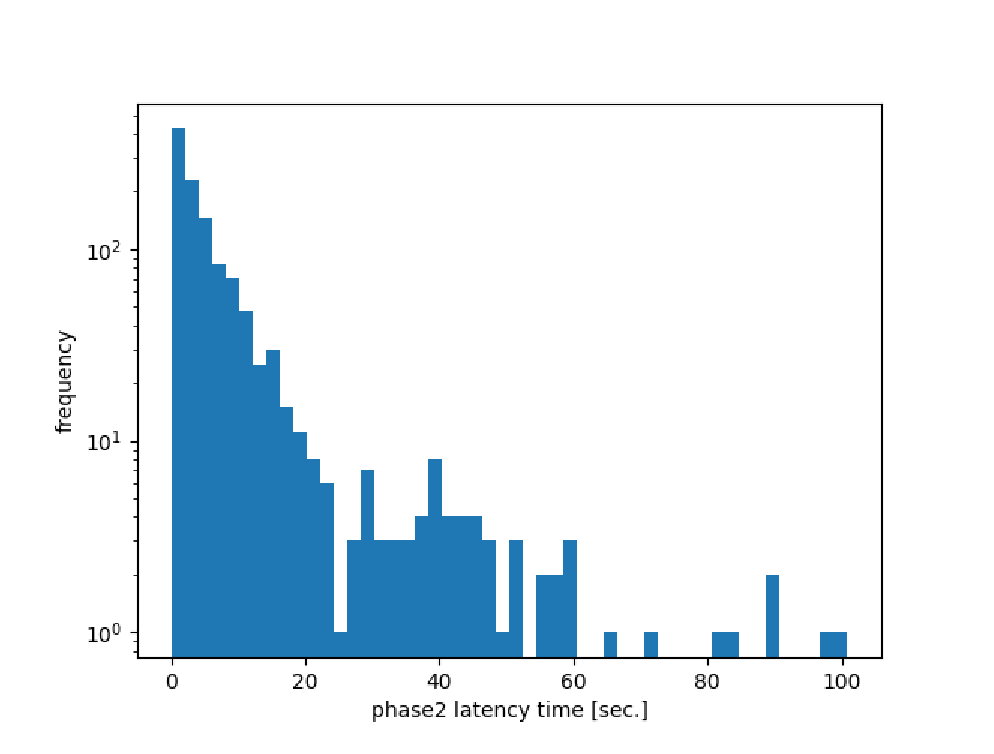
\includegraphics[width=78mm]{pht/phase2-sec-hist.eps}
  \end{center}
  \caption{Phase2の計測時間}
  \label{fig:phase2}
\end{figure}
%
%
\begin{figure}[tb]
  \begin{center}
    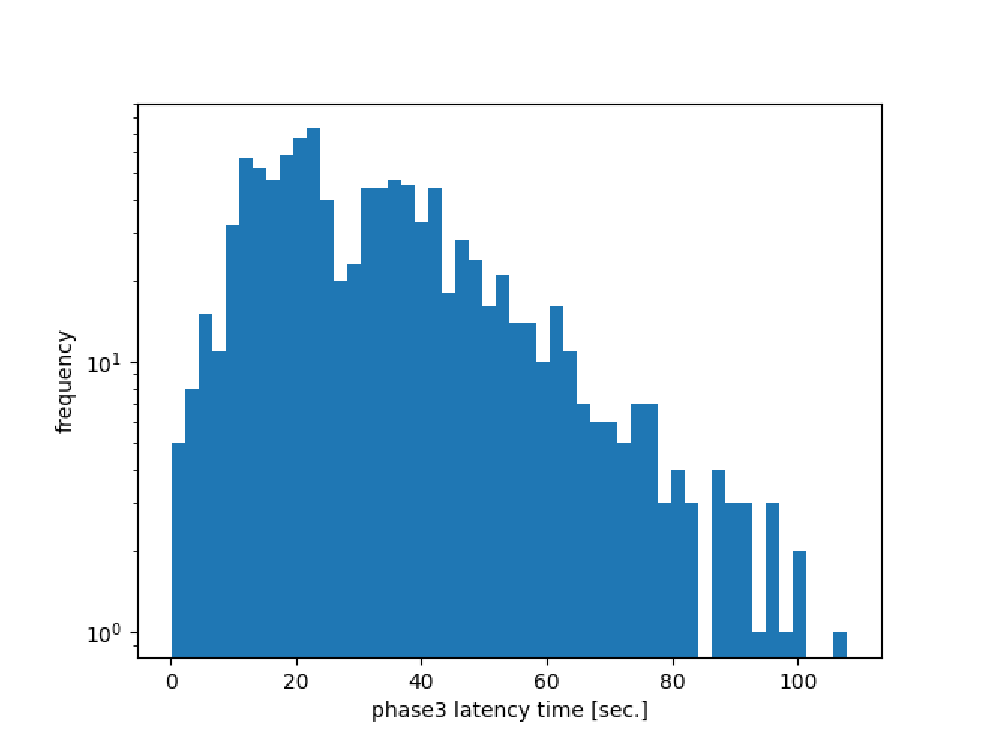
\includegraphics[width=78mm]{pht/phase3-sec-hist.eps}
  \end{center}
  \caption{Phase3の計測時間}
  \label{fig:phase3}
\end{figure}
%
Phase 1は殆どが8秒以下で終わっているが,場合によっては
最悪20秒程度かかることもあることが分かる.
Phase 2はマイニングを行うことから,指数分布に従っている
ことが分かる.
Phase 3は全てのノードのマイニングが完了するのを待つこと
から,タイミングが悪い場合は100秒程度待つ必要があること
が分かる.全てのPhaseを合計すると120秒程度になることか
ら,履歴交差にかかる時間を見積もることができた.

また,1000回の履歴交差のうち,失敗は0回であった.従って,
成功率は100\%となった.

\newpage
%%----------------------------------------------------------------------
\section{まとめと今後の課題}
%%----------------------------------------------------------------------

本研究では,独自のブロックチェーンを管理する複数のドメイン間で
定期的にブロックチェーンの状態を共有することで,互いのブロック
チェーンにヒステリシス署名を書き込み合う履歴交差法を提案した.
提案手法について理論的および実験的観点から,その有効性を評価した.
改ざん耐性の向上比率について理論的に評価した結果,
一般にドメイン数が増加するほど,改ざん耐性向上比率$R$の分布の
ピークが大きい方にシフトすることが分かった.また,ドメイン数が
増えると分布の分散も大きくなることが確認できる.
スケールパラメータ$\alpha=2,3$の比較により,$\alpha$が小さくなる
ほど,改ざん耐性向上比率$R$の分布のピークが小さい方にシフトする
ことも分かった.

次にドメイン間で自律的に通信を行うプロトコルを設計し,実際に
提案法を実行するノードを実装した.実際に履歴交差法にかかる遅延
時間を計測し,その成功率も実験的に評価した.
その結果,120秒程度待つことで履歴交差法の全Phaseが完了すること
が見積もれた.また今回の実験では,履歴交差法の成功率は100\%と
なった.

今後の課題としては,想定される様々な状況においても安定して履歴
交差法が行えるように実験を継続することがある.例えば,履歴交差
を依頼する中心コアノードを固定しない場合,中心コアノードが変化
する場合,履歴交差の依頼が重複してしまった場合への対処,停止
故障を考慮した実装(アルゴリズム2)などが挙げられる.
また,理論的に得られた改ざん耐性向上比率を実験的に評価すること
もある.


\subsection{結果}
\subsection{評価}
\subsection{考察}
\newpage
%%----------------------------------------------------------------------
\section{まとめ}
%%----------------------------------------------------------------------
結論.
#

\newpage
%%----------------------------------------------------------------------
\section*{謝辞}
%%----------------------------------------------------------------------

本研究は,令和2年度修士研究として,千葉工業大学大学院工学研究科電気電子情報工学専攻准教授 藤原明広先生のもとで行ったものである.
本研究を遂行するあたり,適切なご指導,御助言をして頂いた藤原明広先生に深く感謝の意を表する.
同専攻教授 #ーー先生,並びに同専攻教授 #ーー先生には本論文を査読していただき,有益なご意見,コメントを頂いた.ここに感謝の意を表する.
また藤原研究室の各位には,研究遂行にあたり日頃より有益なご討論ご助言を戴いた.
この機会に皆様に深く感謝の意を表す.

\newpage
%%----------------------------------------------------------------------
%% 参考文献
%%----------------------------------------------------------------------

\begin{thebibliography}{99}
\bibitem{Bitcoin}
S.Nakamoto,
``Bitcoin: A Peer-to-Peer Electronic Cash System'' (2008).
\url {https://bitcoin.org/bitcoin.pdf} (2020年1月7日閲覧確認)

\bibitem{fujihara1}
A. Fujihara,
``Proposing a system for collaborative traffic information gathering 
and sharing incentiviz by blockchain technology,''
Advances in Intelligent Networking and Collaborative Systems,
pp.170-182, Springer (2019).

\bibitem{fujihara2}
A. Fujihara,
``PoWaP: Proof of Work at Proximity for a crowdsensing system for 
collaborative traffic information gathering,'' 
Internet of Things, 100046, Elsevier (2019).

\bibitem{suzaki}
洲崎誠一,松本勉,
電子署名アリバイ実現機構 -ヒステリシス署名と履歴交差-
情報処理学会論文誌,Vol.43, No.8, pp.2381-2393, (2002).

\bibitem{saito}
K. Saito,T. Kubo,"BBc-1: Beyond Blockchain One" (2018).
\url{https://beyond-blockchain.org/public/bbc1-design-paper.pdf} (2020年1月7日閲覧確認)

\bibitem{bloX}
bloXroute, \url{https://bloxroute.com} (2020年1月7日閲覧確認)

\bibitem{atomicswap}
Atomic swap, \url{https://en.bitcoin.it/wiki/Atomic_swap#Algorithm}(2020年2月13日閲覧確認)

\bibitem{manabe}
真鍋義文, 「分散処理システム」森北出版 (2013).

\bibitem{hamatsu2018}
濱津誠, 「ゼロから創る暗号通貨」PEAKS出版 (2018).

\bibitem{pings}
WonderNetwork, \url{https://wondernetwork.com/pings}(2020年2月10日閲覧確認)


\end{thebibliography} 

\end{document}
